% Template for PLoS
% Version 3.5 March 2018
%
% % % % % % % % % % % % % % % % % % % % % %
%
% -- IMPORTANT NOTE
%
% This template contains comments intended 
% to minimize problems and delays during our production 
% process. Please follow the template instructions
% whenever possible.
%
% % % % % % % % % % % % % % % % % % % % % % % 
%
% Once your paper is accepted for publication, 
% PLEASE REMOVE ALL TRACKED CHANGES in this file 
% and leave only the final text of your manuscript. 
% PLOS recommends the use of latexdiff to track changes during review, as this will help to maintain a clean tex file.
% Visit https://www.ctan.org/pkg/latexdiff?lang=en for info or contact us at latex@plos.org.
%
%
% There are no restrictions on package use within the LaTeX files except that 
% no packages listed in the template may be deleted.
%
% Please do not include colors or graphics in the text.
%
% The manuscript LaTeX source should be contained within a single file (do not use \input, \externaldocument, or similar commands).
%
% % % % % % % % % % % % % % % % % % % % % % %
%
% -- FIGURES AND TABLES
%
% Please include tables/figure captions directly after the paragraph where they are first cited in the text.
%
% DO NOT INCLUDE GRAPHICS IN YOUR MANUSCRIPT
% - Figures should be uploaded separately from your manuscript file. 
% - Figures generated using LaTeX should be extracted and removed from the PDF before submission. 
% - Figures containing multiple panels/subfigures must be combined into one image file before submission.
% For figure citations, please use "Fig" instead of "Figure".
% See http://journals.plos.org/plosone/s/figures for PLOS figure guidelines.
%
% Tables should be cell-based and may not contain:
% - spacing/line breaks within cells to alter layout or alignment
% - do not nest tabular environments (no tabular environments within tabular environments)
% - no graphics or colored text (cell background color/shading OK)
% See http://journals.plos.org/plosone/s/tables for table guidelines.
%
% For tables that exceed the width of the text column, use the adjustwidth environment as illustrated in the example table in text below.
%
% % % % % % % % % % % % % % % % % % % % % % % %
%
% -- EQUATIONS, MATH SYMBOLS, SUBSCRIPTS, AND SUPERSCRIPTS
%
% IMPORTANT
% Below are a few tips to help format your equations and other special characters according to our specifications. For more tips to help reduce the possibility of formatting errors during conversion, please see our LaTeX guidelines at http://journals.plos.org/plosone/s/latex
%
% For inline equations, please be sure to include all portions of an equation in the math environment.  For example, x$^2$ is incorrect; this should be formatted as $x^2$ (or $\mathrm{x}^2$ if the romanized font is desired).
%
% Do not include text that is not math in the math environment. For example, CO2 should be written as CO\textsubscript{2} instead of CO$_2$.
%
% Please add line breaks to long display equations when possible in order to fit size of the column. 
%
% For inline equations, please do not include punctuation (commas, etc) within the math environment unless this is part of the equation.
%
% When adding superscript or subscripts outside of brackets/braces, please group using {}.  For example, change "[U(D,E,\gamma)]^2" to "{[U(D,E,\gamma)]}^2". 
%
% Do not use \cal for caligraphic font.  Instead, use \mathcal{}
%
% % % % % % % % % % % % % % % % % % % % % % % % 
%
% Please contact latex@plos.org with any questions.
%
% % % % % % % % % % % % % % % % % % % % % % % %

\documentclass[10pt,letterpaper]{article}
\usepackage[top=0.85in,left=2.75in,footskip=0.75in]{geometry}

% amsmath and amssymb packages, useful for mathematical formulas and symbols
\usepackage{amsmath,amssymb}

% Use adjustwidth environment to exceed column width (see example table in text)
\usepackage{changepage}

% Use Unicode characters when possible
\usepackage[utf8x]{inputenc}

% textcomp package and marvosym package for additional characters
\usepackage{textcomp,marvosym}

% cite package, to clean up citations in the main text. Do not remove.
\usepackage{cite}

% Use nameref to cite supporting information files (see Supporting Information section for more info)
\usepackage{nameref,hyperref}

% line numbers
\usepackage[right]{lineno}

% ligatures disabled
\usepackage{microtype}
\DisableLigatures[f]{encoding = *, family = * }

% color can be used to apply background shading to table cells only
\usepackage[table,dvipsnames]{xcolor}

% array package and thick rules for tables
\usepackage{array}

%strikethrough
\usepackage{soul}

%sara: for commenting the pdf to add alt text (if anyone knows a better solution for atl text please help)
\usepackage{pdfcomment}

%Janani: for inserting sparingly few super relevant emojis
\usepackage{emoji} %Rocio: https://www.overleaf.com/learn/latex/Questions/Inserting_emojis_in_LaTeX_documents_on_Overleaf#Emoji_characters_and_the_Overleaf_editor

% create "+" rule type for thick vertical lines
\newcolumntype{+}{!{\vrule width 2pt}}

% create \thickcline for thick horizontal lines of variable length
\newlength\savedwidth
\newcommand\thickcline[1]{%
  \noalign{\global\savedwidth\arrayrulewidth\global\arrayrulewidth 2pt}%
  \cline{#1}%
  \noalign{\vskip\arrayrulewidth}%
  \noalign{\global\arrayrulewidth\savedwidth}%
}

% \thickhline command for thick horizontal lines that span the table
\newcommand\thickhline{\noalign{\global\savedwidth\arrayrulewidth\global\arrayrulewidth 2pt}%
\hline
\noalign{\global\arrayrulewidth\savedwidth}}


% Remove comment for double spacing
%\usepackage{setspace} 
%\doublespacing

% Text layout
\raggedright
\setlength{\parindent}{0.5cm}
\textwidth 5.25in 
\textheight 8.75in

% Bold the 'Figure #' in the caption and separate it from the title/caption with a period
% Captions will be left justified
\usepackage[aboveskip=1pt,labelfont=bf,labelsep=period,justification=raggedright,singlelinecheck=off]{caption}
\renewcommand{\figurename}{Fig}

% Use the PLoS provided BiBTeX style
\bibliographystyle{plos2015}

% Remove brackets from numbering in List of References
\makeatletter
\renewcommand{\@biblabel}[1]{\quad#1.}
\makeatother



% Header and Footer with logo
\usepackage{lastpage,fancyhdr,graphicx}
\usepackage{epstopdf}
%\pagestyle{myheadings}
\pagestyle{fancy}
\fancyhf{}
%\setlength{\headheight}{27.023pt}
%\lhead{\includegraphics[width=2.0in]{PLOS-submission.eps}}
\rfoot{\thepage/\pageref{LastPage}}
\renewcommand{\headrulewidth}{0pt}
\renewcommand{\footrule}{\hrule height 2pt \vspace{2mm}}
\fancyheadoffset[L]{2.25in}
\fancyfootoffset[L]{2.25in}
\lfoot{\today}

%% Include all macros below

\newcommand{\lorem}{{\bf LOREM}}
\newcommand{\ipsum}{{\bf IPSUM}}

%% END MACROS SECTION


\begin{document}

\newcommand{\fede}[1]{\textcolor{ForestGreen}{Fede: #1}}
\newcommand{\rocio}[1]{\textcolor{MidnightBlue}{Rocio: #1}}
\newcommand{\doro}[1]{\textcolor{RedViolet}{Dorothea: #1}}
\newcommand{\jani}[1]{\textcolor{YellowOrange}{Janina: #1}}
\newcommand{\la}[1]{\textcolor{RawSienna}{Laura: #1}}
\newcommand{\as}[1]{\textcolor{Violet}{Andrea: #1}}
\newcommand{\rita}[1]{\textcolor{CarnationPink}{Rita: #1}}

\vspace*{0.2in}

% Title must be 250 characters or less.
\begin{flushleft}
{\Large
\textbf\newline{Ten simple rules to host an inclusive conference} % Please use "sentence case" for title and headings (capitalize only the first word in a title (or heading), the first word in a subtitle (or subheading), and any proper nouns).
}
\newline
% Insert author names, affiliations and corresponding author email (do not include titles, positions, or degrees).
\\
Rocío Joo\textsuperscript{1*}, %,2\Yinyang},
Andrea Sánchez-Tapia\textsuperscript{2},
Sara Mortara\textsuperscript{3},
Yanina Bellini Saibene\textsuperscript{4},
Heather Turner\textsuperscript{5}, %\ddag},
Dorothea Hug Peter\textsuperscript{6}, %\ddag},
Matt Bannert\textsuperscript{7},
Batool Almazrouq\textsuperscript{8},
Liz Hare\textsuperscript{9},
Laura Ación\textsuperscript{10},
Juan Pablo Narváez\textsuperscript{11},
Marcela Alfaro Córdoba\textsuperscript{12},
Federico Marini\textsuperscript{13},
Rita Giordano\textsuperscript{14},
Natalia Morandeira\textsuperscript{15},
Adithi Upadhya\textsuperscript{16},
Joselyn Chávez\textsuperscript{17\Yinyang},
Anicet Ebou\textsuperscript{18\Yinyang},
Silvia Canelón\textsuperscript{19\Yinyang},
Janani Ravi\textsuperscript{20}
%,3\textcurrency}
\\
\bigskip
\textbf{1} Global Fishing Watch, Washington, DC 20036, USA
\\
\textbf{2} Affiliation Dept/Program/Center, Institution Name, City, State, Country
\\
\textbf{3} Affiliation Dept/Program/Center, Institution Name, City, State, Country
\\
\textbf{4} Affiliation Dept/Program/Center, Institution Name, City, State, Country
\\
\textbf{5} Affiliation Dept/Program/Center, Institution Name, City, State, Country
\\
\textbf{6} Affiliation Dept/Program/Center, Institution Name, City, State, Country
\\
\textbf{7} Affiliation Dept/Program/Center, Institution Name, City, State, Country
\\
\textbf{8} Affiliation Dept/Program/Center, Institution Name, City, State, Country
\\
\textbf{9} Affiliation Dept/Program/Center, Institution Name, City, State, Country
\\
\textbf{10} Affiliation Dept/Program/Center, Institution Name, City, State, Country
\\
\textbf{11} Affiliation Dept/Program/Center, Institution Name, City, State, Country
\\
\textbf{12} Affiliation Dept/Program/Center, Institution Name, City, State, Country
\\
\textbf{13} Affiliation Dept/Program/Center, Institution Name, City, State, Country
\\
\textbf{14} Affiliation Dept/Program/Center, Institution Name, City, State, Country
\\
\textbf{15} Affiliation Dept/Program/Center, Institution Name, City, State, Country
\\
\textbf{16} Affiliation Dept/Program/Center, Institution Name, City, State, Country
\\
\textbf{17} Affiliation Dept/Program/Center, Institution Name, City, State, Country
\\
\textbf{18} Affiliation Dept/Program/Center, Institution Name, City, State, Country
\\
\textbf{19} Affiliation Dept/Program/Center, Institution Name, City, State, Country
\\
\textbf{20} Affiliation Dept/Program/Center, Institution Name, City, State, Country
\\
\bigskip

% Insert additional author notes using the symbols described below. Insert symbol callouts after author names as necessary.
% 
% Remove or comment out the author notes below if they aren't used.
%
% Primary Equal Contribution Note
\Yinyang These authors contributed equally to this work.

% Additional Equal Contribution Note
% Also use this double-dagger symbol for special authorship notes, such as senior authorship.
% \ddag These authors also contributed equally to this work.

% Current address notes
% \textcurrency Current Address: Dept/Program/Center, Institution Name, City, State, Country % change symbol to "\textcurrency a" if more than one current address note
% \textcurrency b Insert second current address 
% \textcurrency c Insert third current address

% Deceased author note
% \dag Deceased

% Use the asterisk to denote corresponding authorship and provide email address in note below.
* rocio.joo@globalfishingwatch.org

\end{flushleft}
% Please keep the abstract below 300 words
\section*{Abstract}

The authors of this article recently organized useR! 2021, the annual global R conference, attracting a broad range of participants from academia, industry, government, and the non-profit sector. To embrace the constraints posed by the pandemic, we hosted a 100\% virtual conference. We worked on building a high-quality virtual and global conference by creating a kind, inclusive, accessible, and welcoming environment for everyone. 
This article outlines our most important lessons learned abstracted as `10 simple rules to host an inclusive conference'. These rules apply equally to academic, industry, or mixed conferences; while inspired by a global experience, these rules seamlessly translate to regional events. 
We have designed them for wide adoption to enable and ensure that the scientific and technical conferences are as accessible and inclusive as they can be. 
 

% % Please keep the Author Summary between 150 and 200 words

\linenumbers

\section*{Introduction}

% Rocío: Main message of the paragraph: Conferences are great, but for some
Conferences are spaces to meet and reconnect with members from a specific community, learn about advances in the field, and share our recent contributions.
A good conference experience can be 
However, opportunities for participating in conferences are not equal for all. 
Many academic and tech conferences have become spaces that reproduce systemic inequalities and privileges, i.e. advantages given by society to people from some groups, like being white, male, from a rich country, English-native speaker, with no physical disabilities \cite{arendDisparityConferenceRegistration2019, biggsAcademicConferenceChilly2018, depickerRethinkingInclusionDisability2020a, irishIncreasingParticipationUsing2020}.
% However, conferences are likely to reproduce the systematic discrimination occurring in other spaces in our fields. 

This article proposes 10 simple rules to host inclusive conferences.
They are organized in three sections: \textbf{the pillars}, fundamental rules with key elements to conceive the work on diversity and inclusion in any conference (embracing diversity, creating a welcoming environment, and having a diverse organizing team); \textbf{design rules}, concerning diverse elements in the design of the conference and operational tasks (counteracting bias in the conference program, embracing a strong online component, achieving accessibility for people with disabilities, embracing language diversity, enforcing inclusive communication strategies, and allocating financial resources to support inclusive practices); and a \textbf{process rule} to make the conference part of a long-term commitment to inclusion. 
These practices stem from the experience of organizing useR! 2021, a virtual and global statistical computing conference for users and developers of the R programming language \cite{r_core_team_2021}.
We embraced the challenge of organizing a high-quality virtual conference in the context of the COVID-19 pandemic and making it a kind, inclusive, and accessible experience for as many people as possible.

The authors of this article include the global coordinators of the conference, members of the diversity and inclusion team, and people who contributed to other areas of the conference. We come from different backgrounds, career stages and even continents.
The rules result from our lessons learned from diverse perspectives and expertise. 
Even though these rules were designed based on our experience with a global event, they can be easily transferred or scaled to events with regional or local scopes.
These rules will greatly benefit people who are part of meeting committees that oversee the site/location selection process, or that coordinate with the local organizers of conferences.
The rules will also help organizers who intend to put inclusion at the core of their conference right from the conception and planning phases. We have designed them for wide adoption to enable and ensure that the scientific and technical conferences are as accessible and inclusive as they can be.

% This message is not new. 
% Barriers such as unattainable registration costs, sexism, prejudice against disable people (ableism), among others, have already been exposed and discussed in the literature \cite{arendDisparityConferenceRegistration2019, biggsAcademicConferenceChilly2018, depickerRethinkingInclusionDisability2020a, irishIncreasingParticipationUsing2020}, 
% %timperleyHeMoanaPukepuke2020, gewinWhatScientistsShould2019, brownAbleismAcademiaWhere2018, marks2021meeting
% and some proposals for more inclusive conferences have been put into practice \cite{gichoraTenSimpleRules2010a, levitisCenteringInclusivityDesign2021, atkinsonJournalMedicine20202021, foramittiVirtuesVirtualConferences2021, ninerBetterWhomLeveling2021, rabyMovingAcademicConferences2021, noauthor_discover2021},
% with a primary focus on the online format to open doors for inclusion.\fede{do we need maybe a short definition of the concepts of diversity-equity-inclusion for us/refer to something?} %LA: https://www.cscce.org/resources/organizing-community-events/
% %By inclusion, we mean creating conferences organized by and dedicated to a group of attendees that is representative of the whole population. This means creating a welcoming, respectful, and safe conference that tries to counteract systemic oppression.

% % Rocío: Main message of the paragraph: Roadmap of the paper
% This article focuses on practices for hosting inclusive conferences.
% The rules written here are directed to people who are part of a stable meetings committee that oversees the site/location selection process, or that coordinates with the local organizers of conferences.
% The rules can also be helpful to local/virtual organizers who intend to put inclusion at the core of the planning phase.
% These tips \rita{tips looks to me too informal for an article, maybe used the word `suggestions` or `advice`?} stem from the authors' experience of organizing useR! 2021, a virtual and global statistical computing conference for users and developers of the R programming language \cite{r_core_team_2021}. 
% We embraced the challenge of organizing a high-quality virtual conference in the context of the COVID-19 pandemic and making it a kind, inclusive, and accessible experience for as many persons as possible. 
% Here, we share the lessons learned within the time organizing useR! 2021, summarized as ten simple rules towards hosting an inclusive conference.
% The rules are organized in three groups (Figure \ref{fig:diagram}). %original source: https://docs.google.com/drawings/d/1iS1pLc9OldLMe_jhNT6OGIbT9s5KvlHpUoDd19vHkCY/edit?usp=sharing
% %sara: still need to better format figure size and get the alt text right :P
 
% Group 1 includes rules 1, 2, and 10, which refer to pillars of an inclusive conference: embracing diversity in all its dimensions, creating a safe and welcoming environment for everyone, and making the conference part of a long-term process for inclusion.
% The second group includes rules 3 and 4 and focuses on the people who participate in the conference. 
% Rule 3 refers to the importance of working with an inclusive and diverse organizing team, and Rule 4 concerns the necessity of counteracting implicit and systemic bias from spotlight roles like keynote speakers, other presenters, program committee members, or other session chairs. 
% The third group includes rules 5 to 9. These rules are about components of the conference that should be carefully planned for: an online component, accessibility for people with disabilities, language inclusiveness, a welcoming communication strategy, and financial resources to support inclusion. 
% These rules apply equally to conferences where the expected audience is academic, from the industry, or a mixed group. While these rules are inspired in a global virtual experience they also apply at the regional or local level and can inform in-person and hybrid events.
% \fede{maybe something like: "Even if this set of rules is derived from our experience with a global scale event, we believe these can be easily transferred to events with regional or local scopes"}

\begin{figure}[!h]
\centering
%sara: without success i'm trying to use pdfcomment package and pdftooltip to make the alt-text. any help?
%ast: R/ Unfortunately, support for adding accessibility metadata to LaTeX documents is limited. You will probably need to use Adobe Acrobat to add missing accessibility metadata to your PDF file.https://chi2021.acm.org/for-authors/presenting/papers/guide-to-an-accessible-submission#latex %ast: let's try not to forget this when submitting - some edits to the PDF may be needed to add alt-text to the final version
\pdftooltip{
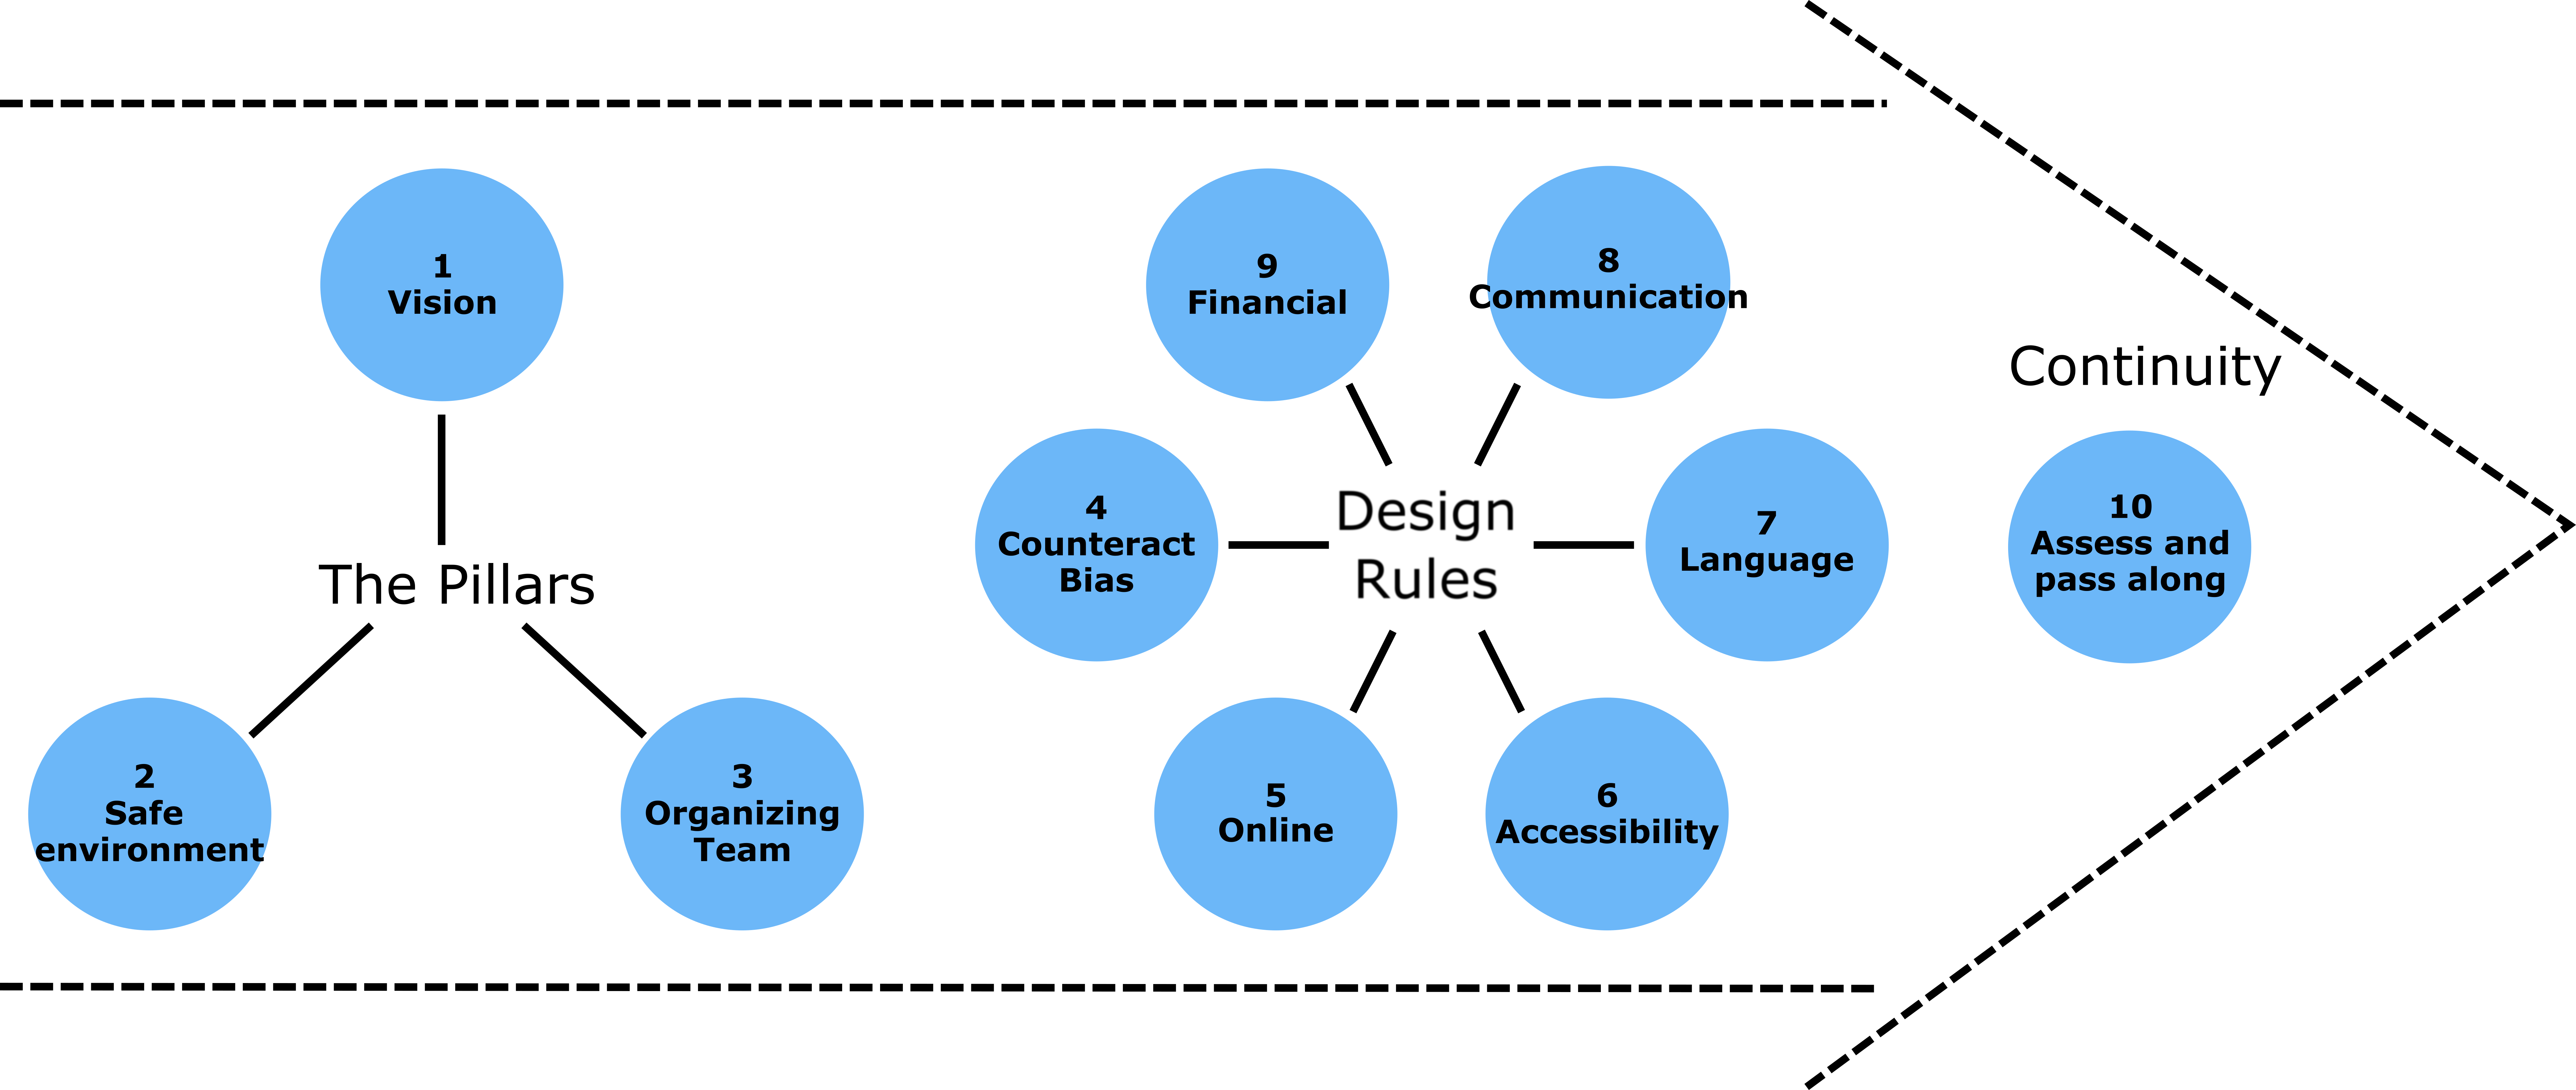
\includegraphics[width=\textwidth]{figs/rules.png}}{
%sara: suggestion for alt text:
%Diagram of how the 10 rules are organized into three groups: grounding rules (rules 1, 2, and 10), people-related rules (rules 3 and 4), and design rules (rules 5 to 9). The diagram has five rows. Each line contains rectangular boxes with the rule number and a short title for each rule. Each rule box is colored based on their group (grounding rules are grey, people-related rules are green and design rules are pink). First row is for the grounding rules 1. Multidimensional diversity and 2. Safe and inclusive environment in grey boxes. Second row is for people-related rules 3. Organizing team and 4. Unbias in green boxes. Third row is for the design rules 5. Online component, 6. Accessibility for disabilities, 7. Language inclusivity in pink boxes. The fourth row is for the design rules 8. Communication and 9. Financial support and budget in pink boxes. The last row is for the grounding rule 10. Diversity and inclusion as a process in grey boxes.
}
\caption{Diagram of the rules organized in three groups: the pillars (rules 1, 2, and 3), design rules (rules 4 to 9), and the process (rule 10).}
\label{fig:diagram}
\end{figure}


\section*{I. The pillars}

To organize a more inclusive conference, it is necessary to identify upfront which groups of people are being excluded, the barriers that keep them from active partaking, and strategies to overcome them. 
\textbf{Rule 1} is about embracing all dimensions of diversity and prioritizing the participation of groups that are often marginalized.
However, increasing diversity alone is not enough. \textbf{Rule 2} focuses on how to create a safe and welcoming environment for all the conference attendees. 
Inclusion should start from the organizing team. \textbf{Rule 3} highlights the importance of starting with an inclusive and diverse organizing team, and provides tips on work dynamics.


\subsection*{Rule 1: Embrace all dimensions of diversity}
\label{rule_diversity}

% Rocío: Main idea: what is diversity and why does it matter? (inequalities)
Diversity encompasses multiple dimensions: age, physical ability, career stage, gender, gender identity, geographic origin, language, neurodiversity, race, religion, sexual orientation, and socioeconomic background, to name a few.
Human diversity should be celebrated and respected in every way. 
Unfortunately, we live in a world with implicit hierarchies along these axes. 
Some statuses (e.g. cisgender, white, male, from North America or Western Europe) hold the privilege of being the defaults around which all systems—including conferences—are consciously and unconsciously built. 
People outside the dominant groups suffer different forms of oppression, like sexism, racism, ableism, homophobia, and transphobia; some of them have to deal with several of these on a daily basis.
% While no isolated initiative can drastically alter xx, building a more diverse and inclusive conference starts by recognizing that these inequalities have systematically excluded whole groups of people from academia and scientific and professional circles. 
Therefore, recognizing this systematic exclusion, particularly in our fields and in our scientific or professional communities, is paramount to inclusion, and will help identify the most marginalized and discriminated subgroups \cite{timperleyHeMoanaPukepuke2020}.
% These are the groups that warrant deliberate efforts that ensure fair inclusion.
As a starting point, the meeting organizers could identify which groups warrant deliberate efforts to ensure fair inclusion, and determine the contributing factors (e.g. explicit discrimination, participation fees).
This analysis should guide the vision of diversity and inclusion for your conference and help design strategies to achieve it. 
Express this vision for your conference in a diversity statement. 
Next, use this vision and the set strategies to define measurable indicators and goals of diversity and inclusion (e.g. a gender distribution of your speakers that is representative of the general population, the presence of racialized people (e.g. Black people) among the organizers, speakers, and attendees, or participation from key geographic regions). 
These numbers should guide you and help achieve your vision.


% realistic but bold (back?)
% be aware and promote awareness
% Rocío: more effort towards including the more excluded
% This may translate into different actions depending on your field, region, or community


\subsection*{Rule 2: Create a safe and welcoming environment}
\label{rule_inclusion}

% Rocío: main idea: Inclusion for everyone
While it is common to think about representation in terms of some of the most visible dimensions of human diversity, such as race, gender, and country of origin, building a genuinely inclusive environment means taking care of all aspects of diversity. %Inclusivity should lie at the heart of setting the tone and meeting space for any meeting as we move forward in the 21st century!
% Edit and make more specific (below)
%\emoji{bulb} \textbf{Practical tips:} 
Here are a few ways in which conference organizers can actively enforce inclusiveness, such as i) Promote respect of pronouns, ii) schedule events exclusive for diverse groups (e.g. LGBTQIA+-friendly spaces), iii) if the conference has an in-person component, pre-assign spaces for religious practices, lactation, and child care, iv) include menu options that account for diverse dietary and religious requirements. These are just a few easy-to-implement examples with a significant impact on including key sub-groups that otherwise find it challenging (see \cite{noauthor_discover2021} for some great advice on `low-hanging fruits').
Importantly, by being proactive in creating such a welcoming space, the organizers can be respectful of attendees' privacy and avoid requiring anyone to disclose personal information, such as revealing a disability, sexual orientation, gender identity, or mental health issues, to name a few.

The organizers should promote a supportive and respectful environment, where all attendants can participate without fear of rejection or isolation. This includes promoting the idea that anyone can act in defense of other attendants in case anything unpleasant, incorrect, of offensive happens. Instead of looking away, act as "active bystanders" and intervene to keep the community safe.
% Rocío: main idea: Code of conduct for a safe place %i think the transition here should leave the two concepts closer. not however. 
However, the most important step that organizers should take to ensure the safety of the community is
Adopting a Code of Conduct (CoC) and gathering a diverse team to enforce it \cite{favaroYourScienceConference2016}.
The CoC is a living document meant to keep the community safe and should state clearly the unacceptable behaviors, the consequences for engaging in such behavior, and the way to report violations \cite{auroraHowRespondCode2019}. 
The CoC team must receive training on how to receive reports, respond to incidents, communicate their responses, and organize protocols on how to respond correspondingly. This should be done during the early phases of the conference planning because CoC violations can happen before the conference too (e.g. social media, organization meetings).  
Since people from marginalized groups are more likely to be victims of Code of Conduct violations and find their claims dismissed due to inadvertent power dynamics, assembling a diverse CoC team will be essential to appropriately deal with discrimination and harassment issues and the power dynamics underneath them with respect and sensitivity. A well-drafted CoC should account for  different cultures and geographical and cultural considerations. 
We strongly recommend reading `How to Respond to Code of Conduct Reports' \cite{auroraHowRespondCode2019} as an excellent starting point for building a strong CoC team.
 


\subsection*{Rule 3: Have an inclusive and diverse organizing team}
\label{rule_organizing_team}

% Rocío: Idea of this paragraph: build a diverse team, and representation

A genuinely inclusive conference can only be organized by an inclusive and diverse team in charge of the conference decision-making.
Organizers should be a team with people from different regions, genders, ethnicities, socioeconomic statuses, and other aspects of diversity.
Having people from diverse backgrounds in decision-making roles will positively affect the conference as a whole because all the processes will benefit from their expertise, experience, and distinct perspectives \cite{hongGroupsDiverseProblem2004}. 
In addition, a diverse team plays an essential role in creating a welcoming space because representation—seeing people with similar life experiences occupy critical positions of power and breaking negative stereotypes—is one of the best ways to create a sense of belonging for everyone participating in the conference (see \textbf{Rule 2} about creating a safe and welcoming environment).

% Rocío: Idea of this paragraph: non-transferability and do not restrict people
People with disabilities often say: `Nothing about us without us' [ref]; the same holds for other dimensions of diversity. The experience of people in marginalized groups facing barriers for equal participation and trying to solve them are invaluable; they cannot be replaced by good intentions or second-hand knowledge from people who have not lived through the same experiences \cite{costanzachockDesign2020}.
% People who have experienced exclusion have the social and technical expertise to fight against it and they will be essential in any team.%ast maybe frame this on a more positive note (ideas, problem solving)
It is important, though, to ensure that organizers with diverse backgrounds are not restricted to only work on diversity and inclusion aspects; 
every member should be granted the freedom to choose which areas of the conference they want to work on, in addition to contributing to decisions involving marginalized communities. 

% Rocío: Idea of this paragraph: tips to make a diverse and inclusive team work + paying them

%\emoji{bulb} \textbf{Practical tips:} 
If you have already started assembling an organizing team, check for gaps in its composition and find representatives accordingly. 
The regional and local communities, groups, or associations in your field are good sources to tap into. 
Furthermore, self-nomination and voting do not always work as reliable mechanisms to fill leadership positions. Instead, it helps to nominate members directly and offer them leading positions in the organization team, especially those that would be typically occupied by people from privileged groups.
Build an environment that encourages healthy conflict and constructive criticism, one in which every person can express their opinion and pay special attention to people from systematically excluded groups.
Many people lack the institutional support to put time and effort into the organization tasks and do not have the luxury to commit to the organization for free; consider paying them as an item in your budget as well as other types of recognition (e.g. public recognition on social media, on the conference website, or during the conference, ideally whatever works best for the contributing member).
Furthermore, tasks such as receiving and responding to Code of Conduct reports can be emotionally intense work and should be additionally rewarded.

% % Rocío: might go to the next rule
% Splitting the workload and responsibilities should not be done by putting care-taking labors--community building, meeting organization and note-taking, conversations with potential partners--on the hands of women and other minoritized groups, while people from privileged groups take the lead in stereotypical highly-valued tasks (see \textbf{Rule \ref{rule_unbias}}). 


\section*{II. Design Rules}

The next set of rules concern diverse elements in the design of the conference and operational tasks. They focus on weaving inclusion into the conference design process.
In \textbf{Rule 4}, we introduce ways to counteract bias in the conference program (keynotes, program committee, abstract selection, and other spaces). 
\textbf{Rule 5} describes the advantages of online conferences by reducing barriers for participation and provides advice for organizing online and hybrid conferences.
\textbf{Rule 6} focuses on best practices to make all conference platforms and spaces accessible to people with disabilities. 
In \textbf{Rule 7}, we advocate for more language-inclusive conferences and provide suggestions to encourage and ensure full participation of non-native English speakers. 
\textbf{Rule 8} provides tips for developing an inclusive media strategy. 
In \textbf{Rule 9}, we address budgeting for inclusive practices, and helping participants with affordable registration costs, scholarships, and other forms of financial support.


\subsection*{Rule 4: Consciously counteract bias in the conference program}
\label{rule_unbias}
%idea of paragraph 1: our lists are biased

When choosing or inviting people for visible and valued roles in the conference –– such as keynote speakers, program/scientific committee, session chairs –– it is likely that there will not be much diversity in the first pool of names.
This is likely due to our inherent biases resulting from existing systems that have always privileged some groups of people \cite{dwyerNoticeWhoScience2021,swartzScienceValueDiversity2019,wongBuildDiversityScience2020,dignazioUnicornsJanitorsNinjas2020}. 
Rather than deter us, this should encourage us to go beyond our narrow and often limited networks to look for, reach out to, invite, encourage, and onboard great people that are not routinely in the spotlight, making sure that these roles do not stay with people in privileged groups (e.g. avoid `manels' and all-white panels; \cite{else_how_2019}; see \textbf{Rule 8}).
\emoji{bulb} It would help to ensure that the composition of all these groups is balanced across topics and areas with representation across regions, gender, race, and career stage, among other aspects.

% our committees are biased and unconscious bias exists
%Having a chance to present at a conference is an opportunity to gain--or keep--visibility in the community or field.

The final list of abstracts making it into the program could also be biased in both submission and acceptance processes. 
For instance, first-time conference participants, especially for the flagship/prestigious meetings, may not feel confident to submit their work.
\emoji{bulb} To counteract this self-selection bias, promote the submission call beyond the usual communication channels and reach out to local groups and communities of practice to encourage submissions by their members.
Some of these communities may have pre-submission mechanisms to help their members receive feedback for their submissions (e.g. the Latin-R and R-Ladies communities have Slack channels to help their members improve their conference abstracts).
On the other hand, the review process may be biased because selection committees — even diverse ones — can be subjected to unconscious or implicit bias.
Unconscious bias happens when we interpret information such as names of the authors, assuming their origin, ethnicity, or their institution of origin, and we attach a positive or negative value to their work according to the stereotypes. Unfortunately, nobody is free from implicit bias \cite{ross_everyday_2020}.
Selection committees need to be gently reminded of such biases with evaluation guidelines (the implicit association test can help identifying them \cite{greenwald_measuring_nodate}) and the organizers need to
identify the most appropriate strategy to counteract them, either with double blind, double open, or single blind reviews \cite{numfocus_discover_2021}.

Double blind reviews can help counteract implicit bias only if the identifying information is completely anonymized in the submission. 
Double open reviews, though more transparent, may still be subjected to implicit bias, and reviewers from minoritized groups might feel additional pressure because the reviews are signed. In this likely case, and in fields where it is not possible to guarantee anonymity of the authors during the selection process (e.g. when non-anonymized GitHub repositories need to be examined), single blind reviews are the only remaining option.  

%\emoji{bulb} \textbf{Practical tips:} 
In any case, design unambiguous evaluation criteria for the submitted proposals that do not put people from minoritized groups at disadvantage (e.g. based on their number of publications or talks), and share them with the authors and reviewers.
Advertising your practices to mitigate bias in proposal selection may also encourage people from diverse groups to submit their work, thus counteracting self-selection bias.

% \cite{swartzScienceValueDiversity2019, wongBuildDiversityScience2020}

% Rocío: main idea: unbias roles and give spotlight to the roles--and people who have contributed in roles--that are not stereotypically categorized as success
Implicit bias also manifests in the weightage given to certain products/activities; e.g. scientific publication and development of software are often rated higher than community building or teaching. 
The latter roles are equally, if not more, challenging and are usually assumed by women, people of color, people with disabilities, and other minoritized groups \cite{cheng2020x+, burfordHomelinessMeantHaving2020}. 
Likewise, research about these topics is undervalued relative to other areas of knowledge production. 
Counteracting bias actively means innovating the program of the conference, proposing new thematic sessions, broadening the scope of talks, keynotes, and tutorials, and giving visibility to the whole range of activities and practitioners that contribute to the overall range and quality of the conference. 


\subsection*{Rule 5: Have a strong online component} 
\label{rule_online}

% Rocío: main idea of the paragraph: online conferences can open opportunities for inclusion
Virtual conferences are more inclusive, removing barriers like costs of registration, transport, accommodation, the logistics of long-distance travel, and discriminatory visa applications \cite{jooKeepOnlineOption2021, ninerBetterWhomLeveling2021, salibaGettingGripsOnline2020, gichoraTenSimpleRules2010a}. 
After experiencing virtual conferences mostly due to the COVID pandemic, there is a widespread call to retain an online component in conferences, either hosting conferences completely virtual or using hybrid formats (combining in-person and online components) \cite{jooKeepOnlineOption2021, woolstonLearningLoveVirtual2020, ninerBetterWhomLeveling2021, roosOnlineConferencesNew2020, levitisCenteringInclusivityDesign2021, sarabipourChangingScientificMeetings2021}.
It is important to note that while being more inclusive, an online component does not guarantee inclusion and accessibility for everyone.
Key decisions must be made early on during the planning phase \cite{levitisCenteringInclusivityDesign2021}. For instance, the chosen conference platforms (e.g. for submission, registration, chatting system, live streaming, etc.) must account for accessibility to accommodate screen-reader users, geopolitical restrictions, and bandwidth requirements. 
\emoji{bulb} The organizers should also decide how to incorporate geographic regions within the schedule of the conference by asking for pre-recorded videos, recording sessions, and sharing them during the conference. Some possibilities for scheduling are: having different days dedicated to different time zones; having each day with the same conference hours, and scheduling time slots that are friendly to different time zones; or having time-zone hubs in each day and repeating the events in each (live for one/few and recorded versions for others). 
A flexible schedule and recorded material will allow many more attendees to partake in the conference, e.g. people with schedules conflicting with the live conference, those who cannot take off, or others who are caretakers. 

% Rocío: main idea: Networking may seem the weakest part of online conference, but it doesn't have to be. 
Networking and socializing have been mentioned as challenging aspects of online conferences, mostly because we are used to in-person interactions at social settings such as coffee or lunch breaks \cite{salibaGettingGripsOnline2020, roosOnlineConferencesNew2020}. 
However, there is evidence that virtual communication can make people from minoritized groups feel more included, thus participate and contribute more \cite{trianaDoesOrderFacetoFace2012,blackEngenderingBelongingThoughtful2020}.

%\emoji{bulb} Practical tips:
Invest time in creating opportunities to meet and bond virtually that can appeal to people with different backgrounds, disabilities, preferences, and remembering that no single networking activity will ever serve the whole community. 
Try new activities centered on different groups of people outside the mainstream of your conference (e.g. \textbf{ABC}); if you think of activities that reach specific groups, preferably co-led by community leaders, these sessions can be more productive, successful, and inclusive.
Some examples are newbies sessions for first-timers, social mixers led by specific subgroups or communities like LGBTQAI+, or leisure activities that reunite subgroups with the same interests: virtual art exhibitions, yoga sessions, movie watch parties, trivia quizzes, shared language, etc. 
Offer activities that require voice or video interactions, and others that involve only written chat, and make all participation optional and voluntary.

If you are organizing a hybrid event instead, you should decide on the relative importance that the online and in-person components will take. The most inclusive practice would be to give equal weight to both components, articulating them well and maximizing the experience of everyone attending your conference regardless of the preferred format \cite{bajpai_towards_2021}. 

\emoji{bulb} For this format, the audience, chairs, and presenters -- of talks, posters, and workshops -- could be either in-person or remote, and they should all be able to interact. 
To best include both kinds of attendees, all questions and comments should pass through an online system, or have an pre-designated point person who enables this cross-talk. 
The physical venue would have to include multiple ways to connect with online folks such as tablets on the meeting venue, cameras and microphones that allow online attendants to follow who is speaking at the in-person space.
This requires the venue to have stable and secure internet connection for the in-person participants to join the online folks. 
Having a hybrid format also means accounting for the fact that the venue does not need to host all the attendees. You should estimate in advance how many in-person attendees to expect, and ask them early on during registration or pre-registration. This could save you time and money when looking for a suitable venue.
When planning for networking activities in hybrid events, use the same principles outlined above and offer various activities engaging different groups. It is understandable that a few of these activities could be only in-person, but to promote connections between both groups of participants, there should be a fair proportion of activities connecting in-person and online attendees. 


\subsection*{Rule 6: Make the conference accessible to people with disabilities}
\label{rule_accessibility}

% Be more direct
Conferences are among the least accessible spaces that people with disabilities may encounter in professional contexts \cite{priceAccessImaginedConstruction2009}. Even when conferences implement other inclusive practices, the participation of people with disabilities is often overlooked \cite{marks2021meeting}. Including people with disabilities in the organizing team can have a large impact from the beginning (see \textbf{Rule 3}), since planning for accessibility requires time, experience, and early decision-making \cite{irishIncreasingParticipationUsing2020}. As other aspects of inclusion, dealing with accessibility at the last minute is the recipe for a disastrous conference. If you do not consider accessibility from the conference inception, it is highly likely that you will be better off without trying to patch accessibility at the last minute. Key decisions in this respect are hard to correct.

If the conference has an in-person component, the venue should comply with common accessibility standards, such as being adequate for people who use wheelchairs, have signs in Braille, and a sound system compatible with hearing devices and live interpretation, just to name a few important features. In addition to this, the organizers should take care proactively of invisible disabilities (e.g. dyslexia, anxiety, ADHD, autism). This could be done in many ways, for example, by providing quiet spaces for privacy and noise-free conversations, or providing chairs in open spaces.

Regardless of the conference format, all platforms (website, chat, conference administration tools) and images used for the communication strategy of the conference should be screen-reader friendly, keyboard accessible, and have alternative text. Every video should have good-quality (not automated) captions and a transcript; live presentations should have good-quality captions too. 
Provide accessibility guidelines for slides and presentations, encourage their use, and be available for any questions presenters and attendees may have. For instance, useR! 2021 published accessibility guidelines for every format of the conference, a blog post with recommendations, and two post-conference blog posts regarding the whole accessibility experience. The participation of a blind person in the organizing team was key to several of these decisions. 
Slide decks should be made available beforehand, either in webpages or available for download to ensure that everybody can follow their content during the presentations. 

Accessibility practices should cover social events and networking, which should include activities that do not restrict participation based on body type or ability. 

Importantly, all these accessibility practices are inclusive not only for people with disabilities but to everyone.
For instance, captions are helpful for non-native speakers, having the material available for download helps attendees with low bandwidth connection, etc. Accessibility efforts should be explicitly displayed in the official communication channels and inform potential attendees with disabilities a point of contact to solve any questions in this respect.
Clear communication about the lack of accessibility of some spaces or activities is also highly recommended, to give a clear notion of the conference experience (see \textbf{Rule 8} about communication strategy).

\subsection*{Rule 7: Include languages other than English}
\label{rule_language}

% Rocío: main idea: English as the only language makes some people privileged and is a barrier for others
In international meetings, the linguistic diversity of the participants is often overlooked. 
English is usually the official and sole language for submissions, presentations, tutorials, workshops, conference platforms, webpages, and communications. 
While English is indeed regarded as the primary language in scientific communication and one official language makes it conducive to communicate widely, this makes being a native English speaker a privilege.%RJ: Could cite Amano's paper here.
Non-native English speakers could miss opportunities to attend or actively participate in conferences (e.g. asking questions or participating in discussions),
and conferences may in turn miss innovative contributions.


% Rocío: main idea: make conferences more linguistically inclusive
Providing a welcoming and diverse environment by encouraging the full participation of non-native English speakers is critical (\textbf{Rule 2} about a welcoming environment for all). This may be done at different levels.
Allow for abstract submission in both English and the language the person feels more comfortable with, and consider the possibility of assigning a reviewer who is fluent in that language. That way, the abstract will be judged primarily by the quality or relevance of the work instead of the English grammar.
For presentations spoken in English, provide English-to-English captions to help non-native English speakers (in addition to people with hearing disabilities) follow the presentations. Whenever possible, identify other key languages for the conference and provide translated captions or live interpretation into these key languages, including multilingual Q \& A sessions.
The following step would be having sessions and events in languages other than English, both regarding the technical content of the conference and the social and networking aspects. Networking sessions in languages other than English can include captions, interpretation or none of them; the latter has the benefit of not requiring additional technical adjustments. 
Keynotes and regular talks should always be accompanied by captions or live interpretation to English.
Promote the attendance to presentations in languages other than English as key components of your schedule and announce when captions are available. 
Remind your native English speaking audience to be respectful of accents and mistakes in English. 


% Rocío: we could eventually cite https://conferenceinference.wordpress.com/2020/11/30/when-language-is-not-a-barrier-a-tale-fr[…]istically-inclusive-conference-toma-pustelnikovaite/


\subsection*{Rule 8: Convey the welcoming spirit in your communication strategy}
% media
\label{rule_communication}

%Rocío: Main idea: Include people in your communication 
The communication strategy of your conference should aim to increase the number and diversity of participants, and be inclusive by design.
Actively reach out and promote the conference to communities that have been systematically excluded. 
Publish the diversity statement, Code of Conduct, accessibility guidelines, and options for financial support (see \textbf{Rule 9} about financial resources) to emphasize that everybody is welcome to join the event.
Try to develop creative ways to show that everyone is seen, respected, and welcome. For example, useR! 2021 created a mascot for the conference wearing different scarves reflecting folks from various minoritized groups that the conference wanted to reach (\textbf{Fig. 2}). 
The diverse members of your team should be able to decide which languages to emphasize and which social media platforms to utilize for the promotion of the conference (e.g. Twitter, Facebook, LinkedIn, conference website, mailing lists).
Be transparent with potential attendees and communicate limitations of your conference to let them know what to expect, and ways in which you will try to mitigate these issues. For instance, inform if the conference platform is not completely screen-reader friendly, let people know if you are offering personalized help to navigate it, or if captions will be available for some talks but not all.

%Rocío: Main idea: Use inclusive language
\emoji{bulb} Inclusive language — language free from words, phrases, or tones that reflect prejudiced or discriminatory views of particular people or groups — should be used in all communications \cite{hallDesigningDiversityInclusion2019}. 
Become familiar with the terminology used for disabilities, racialized groups, gender and sexual orientations, and other terms that should be avoided. %
Do not expect minoritized people to teach you—it's not their role—, and accept feedback without being offended.
Inclusive language also encompasses avoidance of excessive and too specific technical jargon and acronyms. 
% links, examples, this changes with the context
%practice: create a standards in inclusive language for your community, to build collective knowledge than can be passed to 


\begin{figure}[!h]
\centering
\pdftooltip{
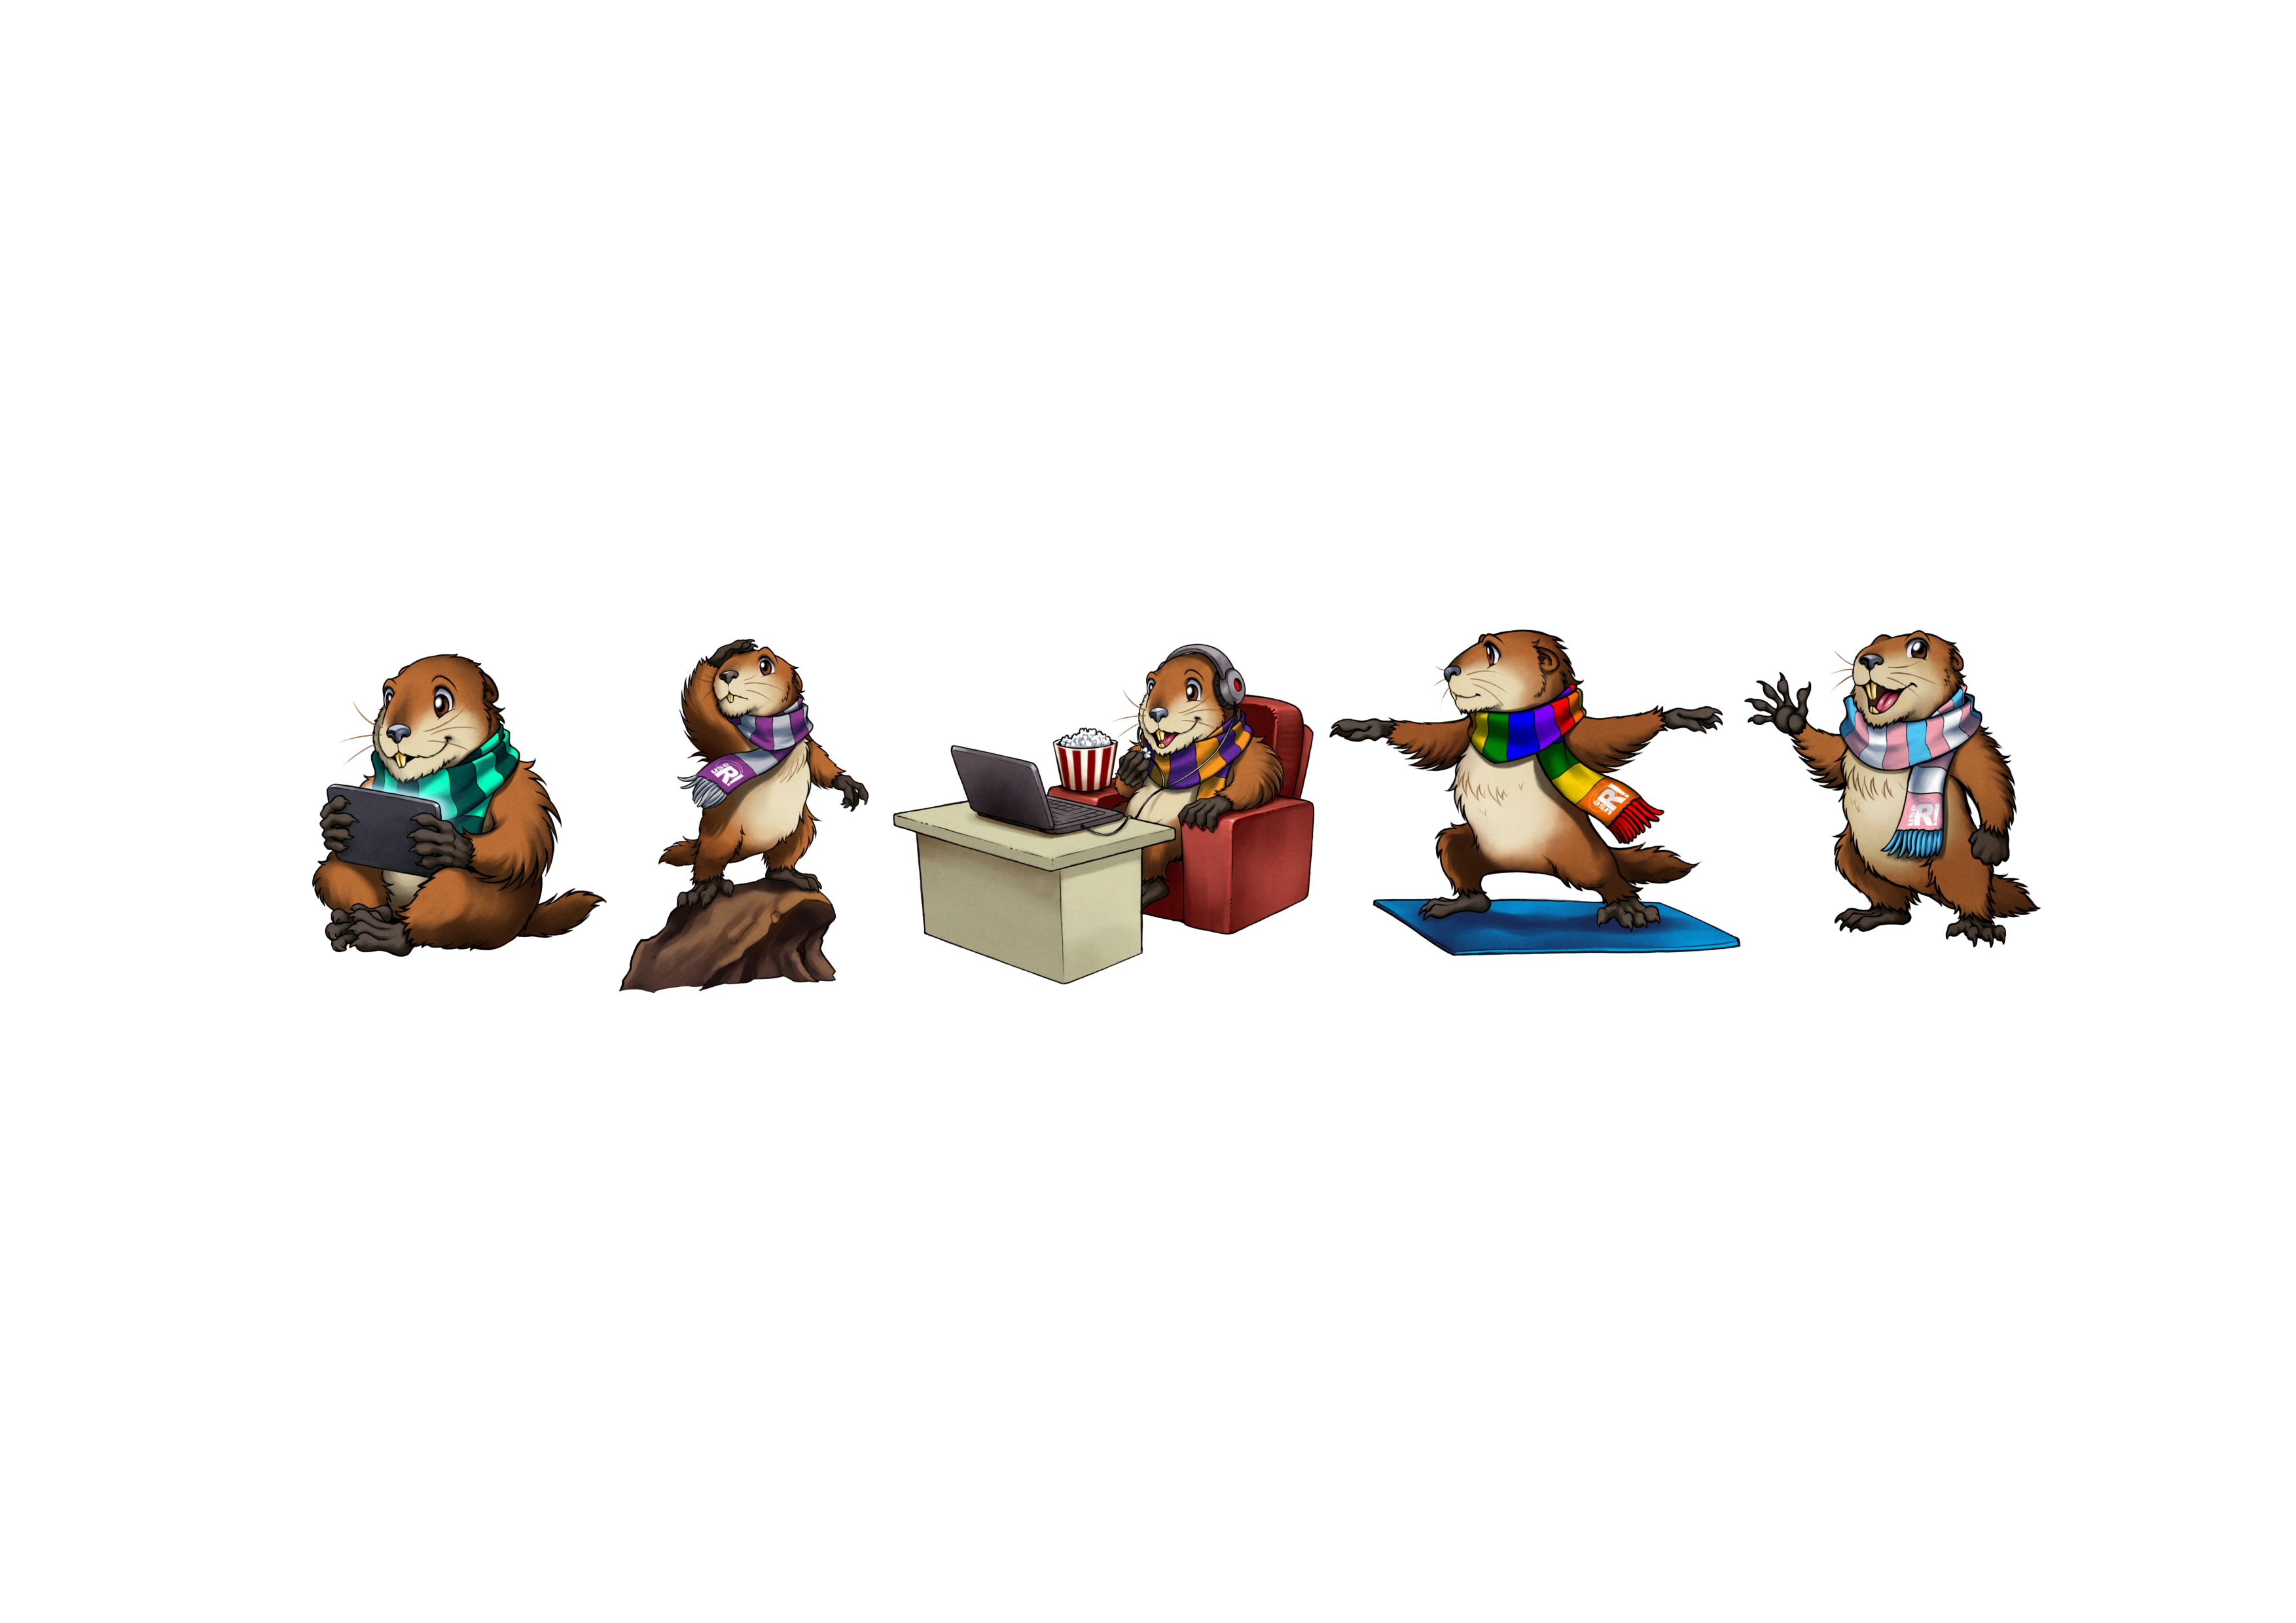
\includegraphics[width=\textwidth]{figs/marmots.pdf}}{
}
\caption{Margot the marmot was useR! 2021 mascot. To represent the global and inclusive nature of the conference, Margot was drawn using scarves representing diverse groups that are part of the large R community: (from left to right) MiR (Minorities in R), LGBTQAI+, R-Ladies, transgender people, and AfricaR.} %RJ: Need to acknowledge Francisco's contribution.
\label{fig:marmots}
\end{figure}

\subsection*{Rule 9: Allocate adequate financial resources to support your conference goals}
\label{rule_financial}

% Rocío: main idea: Need to budget for inclusive practices.
Allocation of resources to support the goals of inclusion of the conference has to be intentional. 
Estimate the costs for these practices and define your priorities in advance (e.g. paying the organizing team, Code of Conduct training, captioning).
Additional support for attendees could also be considered in the budget: child care support, transportation fees, visa-related support (if in-person), internet connection services (for the virtual component). 
Consider that an online conference might reduce organization costs (e.g. no rental costs for a physical venue), allowing to redirect the money towards other inclusive priorities. 
When asking for sponsorship, it might be easier to justify supporting concrete actions towards inclusion than making generic demands for funding.


% Rocío: main idea: help take the burden out of participants for more inclusive participation
When determining the registration rates, the socioeconomic context of participants, their country of origin, and their career status should be taken into account  \cite{sarabipourChangingScientificMeetings2021, andalibPostdocQueueLabour2018, kaplanPostdocNot2012}
(see \cite{canelon2021cost} for an example of conversion rates based on country of origin and career status). 
Resources permitting, allow the possibility of a 'pay what you can' option. You could also aim to have a conference with no registration costs; this is especially true for online events, but bear in mind that free events have a lower attendance rate than paid events \cite{eventbrite_ultimate_2017}. 
%Other costs can be prohibitive-> scholarships
Scholarships to attend the in-person component of the conference are an additional way to boost participation of people from marginalized groups, by offering support for travel and lodging expenses.
Design the diversity-related scholarship to be explicit about the groups you want to support, and be transparent about the criteria for evaluation to avoid self-selection (refraining from applying because they think they don't stand a chance). 
Conferences usually ask for cover letters or applications to assign these scholarships, which can be time-consuming and emotionally demanding. 
\emoji{bulb} Simplifying and deconstructing the process of requesting financial support, especially for 
people who lack the time and resources (e.g. because they have family responsibilities) might greatly improve the probability of minoritized participants applying for the much-needed support. 
Bear in mind that transferring money internationally is a cumbersome administrative process that can significantly augment the burden of already marginalized groups. Whenever possible, facilitate alternate ways for money transfer (e.g. book flights, hotel reservations, waive conference fees).



\section*{III. The Process}

A conference is a critical community-building space, and can foster change in future events and the community itself. The organizers of a conference edition and members of selection committees should do their best to pass along their knowledge on best practices and problems encountered to future organizers.


\subsection*{Rule 10: Make the conference part of a long-term process for inclusion}
\label{rule_process}

% Rocío: main idea: assess how inclusive was the conference
As conference organizers, one of the key post-conference tasks is to analyze conference attendee, participant, and organizer data including their experiences. It is essential to assess whether equity and inclusion goals were met during the conference, as a result of the steps taken. 
\emoji{bulb} You can rely on the diversity indicators defined at the beginning of the planning process (\textbf{Rule 1}). 
It is likely that you will be able to calculate some of your indicators directly from information that you have already collected from your organizing team, speakers, and participants (e.g. countries of origin, or preferred language).
Other indicators may need a special survey asking for additional information and feedback about the conference. 
In the survey, providing options for open answers will allow people to express their opinions freely, and may give you more insights into how/why your inclusion practices worked or not. 
% Do not expect everything to be perfectly inclusive, or to encompass all the dimensions of diversity at once. %You're part of a process and contributing to structural change.

% Pass the information
%\emoji{bulb} Practical tips
Document your processes, outcomes, and lessons learned through blog posts, reports, and presentations. 
Make sure you share this information with future organizers, as well as the contact information of the people you worked with (if they agree to it), to give them a good well-informed baseline to improve inclusion in the following editions of the conference.
If you are part of a stable meeting committee (overseeing multiple editions), encourage organizers to follow these Rules and set up new standards for inclusion: be explicit on the inclusive spirit of the conference and the practices that future organizers should commit to when publishing the call for conference organization and the selection criteria. 
%something about the past - shoulder of people before, federico


\section*{Concluding remarks}

This article suggests changes in conference planning towards diversity and inclusion. 
Organizing a conference and implementing inclusive practices are both learning experiences.
As conference organizers, we started with different levels of clarity about the principles and practices described here, learned many of them together during the organization phase, and learned even more when translating them into ten rules for this paper. 
We hope that they can be useful guidelines to improve diversity and inclusion in your conference.  
And that you can adapt them, improve them, and share your lessons and experience with as many people as possible. 

Be aware of all the factors that may hinder your efforts for inclusion: systemic discrimination, time or money constraints, geopolitical or public health contexts, personal issues affecting your organizing team. 
Try to account for these factors as best as you can to set realistic yet bold vision and goals of diversity and inclusion for the conference.
At the end of the day, even if you do not achieve them at 100\%, striving for them will make you stretch what feels possible and help you make changes you would have otherwise not even attempted to make. 
And most importantly, you would have contributed to a great conference experience for the attendees. 
They will notice the welcoming and inclusive spirit of the conference reflected in the pillar rules, and translated into design decisions—even if there are gaps in them due to the constraining factors mentioned above. 
Inclusive conferences can help to enhance career paths and create a sense of belonging in the community. 
That is more than enough motivation to make the effort worth it. 


\section*{Authors' contributions}

To list author contributions, we used the high-level contributor roles in the CRediT framework relevant for this study (project administration, supervision, writing original draft, conceptualization, writing—major reviews and edits, resources, and visualization; \url{http://credit.niso.org}), and an additional category for contributions on their own ten simple rules for an inclusive conference without looking at the first draft (i.e. sharing rules).

\begin{itemize}
    \item RJ: Project administration, Supervision, Writing original draft, Conceptualization, Writing--major reviews and edits, Resources, Visualization
    \item AST: Project administration, Supervision, Conceptualization,  Writing--major reviews and edits, Resources, Visualization, Sharing rules
    \item SM: Conceptualization, Writing--major reviews and edits, Resources, Visualization, Sharing rules
    \item YBS: Conceptualization, Writing--major reviews and edits, Resources
    \item HT: Conceptualization, Writing--major reviews and edits, Resources
    \item DHP: Conceptualization, Writing--major reviews and edits, Sharing rules
    \item MB: Conceptualization
    \item BA: Writing--major reviews and edits, Resources, Sharing rules
    \item LH: Writing--major reviews and edits, Resources, Sharing rules
    \item LA: Writing--major reviews and edits, Resources
    \item JPN: Writing--major reviews and edits, Visualization
    \item MAC: Writing--major reviews and edits
    \item FM: Writing--major reviews and edits
    \item RG: Writing--major reviews and edits
    \item NM: Sharing rules
    \item AU: Sharing rules
    \item JC: Sharing rules
    \item AE: Sharing rules
    \item SC: Sharing rules
    \item JR: Writing--major reviews and edits
\end{itemize}



\section*{Acknowledgments}
The authors of this piece would like to thank every single member of the organizing team of useR! 2021 [ \url{https://user2021.r-project.org/about/global-team/}] for their valuable contribution to an inclusive conference experience, and the R Foundation for trusting us with the organization of useR! 2021 and supporting us through the process. 


% \nolinenumbers

% % Either type in your references using
% % \begin{thebibliography}{}
% % \bibitem{}
% % Text
% % \end{thebibliography}
% %
% % or
% %
% % Compile your BiBTeX database using our plos2015.bst
\bibliography{community-science}
% % style file and paste the contents of your .bbl file
% % here. See http://journals.plos.org/plosone/s/latex for 
% % step-by-step instructions.
% % % 
% \begin{thebibliography}{10}

% \bibitem{bib1}
% Conant GC, Wolfe KH.
% \newblock {{T}urning a hobby into a job: how duplicated genes find new
%   functions}.
% \newblock Nat Rev Genet. 2008 Dec;9(12):938--950.

% \bibitem{bib2}
% Ohno S.
% \newblock Evolution by gene duplication.
% \newblock London: George Alien \& Unwin Ltd. Berlin, Heidelberg and New York:
%   Springer-Verlag.; 1970.

% \bibitem{bib3}
% Magwire MM, Bayer F, Webster CL, Cao C, Jiggins FM.
% \newblock {{S}uccessive increases in the resistance of {D}rosophila to viral
%   infection through a transposon insertion followed by a {D}uplication}.
% \newblock PLoS Genet. 2011 Oct;7(10):e1002337.

% \end{thebibliography}



\end{document}

